\section{Data and simulated samples}\label{chap6:datatsets}

The data sets, triggers, pile up reweighting, lepton identification and isolation used in this analysis are the same as the SM Higgs search and are described in Sec.~\ref{chap5:dataset}.

Also, the same MC simulations are used for the background processes, the only exception being the DY background, for which the \textsc{MG5\_aMC@NLO} generator is used with LO QCD accuracy, matching together events with up to four jets in addition to the vector boson with the MLM~\cite{Alwall:2007fs} matching scheme. Given that this analysis aims to probe regions of phase space where the DY contribution is very small, like in the high transverse mass region, the usage of a simulation of the inclusive DY process may lead to large uncertainties due to the limited simulation statistics in the sample. To partially overcome this issue, different DY samples are generated in restricted portions of the phase space defined by the $H_\mathrm{T}$ variable, i.e. the scalar sum of all the partons \pt in the event. For $H_\mathrm{T}< 100$\GeV the inclusive simulation is used, while different samples are used for higher values of $H_\mathrm{T}$. The samples are merged using the parton level information, and it has been verified that a smooth transition between different $H_\mathrm{T}$ regions is achieved, as shown in Fig.~\ref{fig:DY_HT}.
The DY LO cross section obtained from the simulation is scaled using the LO to NNLO k-factor of 1.23.

\begin{figure}[htbp]
\centering
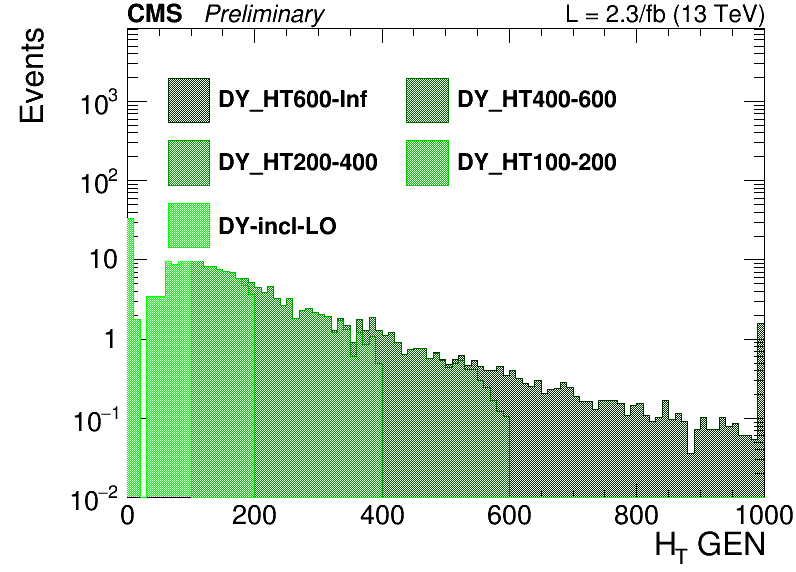
\includegraphics[width=0.5\textwidth]{images/13TeV/log_c_incl_HTGen.png}
\caption{
    Generator level $H_\mathrm{T}$ distribution for the merged DY sample.}
    \label{fig:DY_HT}
\end{figure}

In order to perform the resonance search in a large part of the mass spectrum, several signal samples for the gluon-gluon fusion and the vector boson fusion mechanisms have been generated corresponding to different Higgs boson masses in the range between 200\GeV and 1\TeV. The signal width for each mass point corresponds to the one expected for a SM Higgs boson at that mass. The samples are produced with a mass step of 50\GeV from 250 to 800\GeV and of 100\GeV from 800 to 1000\GeV. A finer stepping is used between 200 and 250\GeV. All the signal samples are generated with the \textsc{Powheg V2} generator, interfaced with the \textsc{JHUGen v6.2.8} generator, which handles the decay of the Higgs boson to $\mathrm{W^+ W^-}\to2\ell2\nu$.

The interference effects among gg$\to$X$\to$WW, gg$\to$WW and gg$\to$H$\to$WW are evaluated using the  \textsc{mcfm} and \textsc{JHUGen} generators, as implemented in the MELA (Matrix Element Likelihood Approach) framework~\cite{JHUGen}. Details about the interference effects are given in Sec.~\ref{chap6:AnalysisStrategy}.
